Die Funktion
\[
\varphi(x)
=
\begin{cases}
0&\qquad x\le -1\\
a\sqrt{x+1}&\qquad -1<x\le 0\\
a\sqrt{1-x}&\qquad 0<x\le 1\\
0&\qquad x>1
\end{cases}
\]
soll als Wahrscheinlichkeitsdichte einer Zufallsvariable $X$ verwendet werden.
\begin{center}
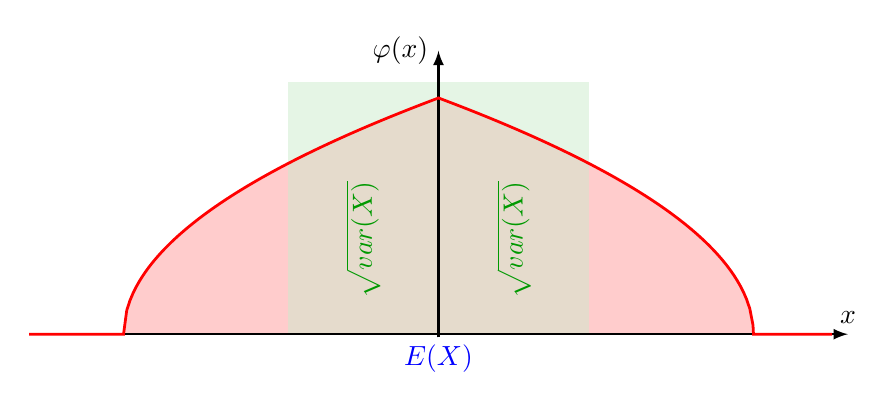
\begin{tikzpicture}[>=latex,thick,scale=4]
\definecolor{darkgreen}{rgb}{0,0.6,0}
\def\a{0.75}
\fill[color=red!20]
	(-1,0)
	-- plot[domain=-1:0,samples=100] ({\x},{\a*sqrt(\x+1)})
	-- plot[domain=0:1,samples=100] ({\x},{\a*sqrt(1-\x)})
	-- (1,0) -- cycle;
\ifthenelse{\boolean{pruefung}}{}{
\fill[color=darkgreen!20,opacity=0.5]
	({-sqrt(8/35},0) rectangle ({sqrt(8/35)},0.8);
\node[color=darkgreen] at ({-0.5*sqrt(8/35)},0.3) [rotate=90]
	{$\sqrt{\operatorname{var}(X)}$};
\node[color=darkgreen] at ({0.5*sqrt(8/35)},0.3) [rotate=90]
	{$\sqrt{\operatorname{var}(X)}$};
\draw[color=blue,line width=1pt] (0,-0.01) -- (0,0.8);
\node[color=blue] (0,0) [below] {$E(X)$};
}
\draw[->] (-1.3,0)  -- (1.3,0) coordinate[label={$x$}];
\draw[->] (0,-0.01) -- (0,0.9) coordinate[label={left:$\varphi(x)$}];
\draw[color=red,line width=1pt] (-1.3,0)
	-- (-1,0)
	-- plot[domain=-1:0,samples=100] ({\x},{\a*sqrt(\x+1)})
	-- plot[domain=0:1,samples=100] ({\x},{\a*sqrt(1-\x)})
	-- (1,0) -- (1.25,0);
\end{tikzpicture}
\end{center}
\begin{teilaufgaben}
\item
Wie muss $a$ gewählt werden, damit $\varphi$ wirklich eine
Wahrscheinlichkeitsdichte ist?
\item
Bestimmen Sie den Erwartungswert $E(X)$
\item
Bestimmen Sie die Varianz $\operatorname{var}(X)$
\end{teilaufgaben}

\thema{Wahrscheinlichkeitsdichte}
\thema{Erwartungswert}
\thema{Varianz}

\begin{loesung}
\begin{teilaufgaben}
\item
Es muss gelten
\[
1
=
\int_{-\infty}^\infty \varphi(x)\,dx
=
\int_{-1}^0 a\sqrt{x+1}\,dx
+
\int_0^1a\sqrt{1-x}\,dx
\]
Da $\varphi(x)$ symmetrisch ist bezüglich $0$ reicht es, nur eines der
Integrale auszurechnen.
Dazu führt man eine Variablentransformation $t=1-x$ aus:
\begin{align*}
\int_0^1a\sqrt{1-x}\,dx
&=
-a\int_1^0 \sqrt{t}\,dt
=
a\int_0^1 t^{\frac12}\,dt
=
a\biggl[\frac23 t^{\frac32}\biggr]_0^1
=
\frac{2a}3.
\\
\int_{-\infty}^\infty\varphi(x)\,dx
&=
\frac{4a}{3}
=
1
\qquad\Rightarrow\qquad
a=\frac{3}{4}.
\end{align*}
\item
Da die Funktion $\varphi(x)$ symmetrisch ist, ist der Erwartungswert $E(X)=0$.
\item
Für die  Varianz brauchen wir zunächst $E(X^2)$:
\begin{align*}
E(X^2)
&=
\int_{-\infty}^\infty x^2\varphi(x)\,dx
=
2a\int_0^1 x^2\sqrt{1-x}\,dx
\\
&=
-2a\int_1^0 (1-t)^2\sqrt{t}\,dx
=
2a\int_0^1 t^{\frac12}-2t^{\frac32}+t^{\frac52}\,dt
\\
&=
\frac32\biggl[
\frac23 t^{\frac32}
-2\frac25 t^{\frac52}
+\frac27t^{\frac72}
\biggr]_0^1
=
\frac32\biggl(
\frac23 - \frac45+\frac27
\biggr)
=
1-\frac65+\frac37
=
\frac{35-42+15}{35}
=
\frac{8}{35}.
\end{align*}
Da $\operatorname{var}(X)= E(X^2) - E(X)^2=E(X^2)=\frac{8}{35}\approx0.22857$ haben wir damit
auch schon die Varianz gefunden.
\qedhere
\end{teilaufgaben}
\end{loesung}

\begin{bewertung}
\begin{teilaufgaben}
\item
Normierungsbedingung ({\bf N}) 1 Punkt,
Wert für $a$ ({\bf A}) 1 Punkt.
\item
Wert des Erwartungswertes ({\bf E}) 1 Punkt.
\item
Integralformel für $E(X^2)$ ({\bf I}) 1 Punkt,
Varianzformel $\operatorname{var}(X) = E(X^2)- E(X)^2$ ({\bf V}) 1 Punkt,
Wert der Varianz ({\bf W}) 1 Punkt.
\end{teilaufgaben}
\end{bewertung}
